\chaptertitle{第一章\quad 平面上的几何变换}

本书的第一章从一个最简单的问题开始：在坐标平面上，如果我们把每个点按照某种规则挪到一个新的位置，整个图形会发生什么变化？旋转一下、翻折一下、拉长一下、推挤一下——这些在日常生活中用手就能比划的"动作"，进入数学之后就变成了精确的坐标公式。本章逐一考察五种最基本的几何变换，用大量具体数字建立直觉，最后你会发现它们竟然都写成同一种形式——这将是第二章引出"矩阵"概念的伏笔。

\sectiontitle{1.1\quad 坐标——给平面上的点一个"地址"}

取一张方格纸。在纸上画两条互相垂直的直线：水平的这条叫$x$轴，竖直的这条叫$y$轴。两条线相交的那一点叫原点，记作$O$。

现在平面上任何一个点都可以用两个数来"定位"。从原点到那个点，向右（或左）走多少格给一个数，向上（或下）走多少格再给一个数。向右和向上的方向为正，向左和向下的方向为负。这两个数分别叫该点的$x$坐标和$y$坐标，记作$(x,y)$。

\begin{example}
写出以下各点的坐标：
(1) 从原点向右2格、向上5格；
(2) 从原点向左3格、向下1格；
(3) 从原点向左4格、向上0格。
\end{example}
\begin{solution}
(1) 向右为正、向上为正，所以是$(2,5)$。\\
(2) 向左为负、向下为负，所以是$(-3,-1)$。\\
(3) 向左为负、向上为0，所以是$(-4,0)$。
\end{solution}

有了坐标，平面上的任何一个图形都可以用它的顶点的坐标来描述。比如一个正方形，四个顶点可能是$(0,0)$、$(2,0)$、$(2,2)$、$(0,2)$。直线的方程也可以写成坐标形式。

\textbf{变换}是什么？就是把平面上的每个点$(x,y)$按照一定的规律挪到一个新的位置$(x',y')$。挪完了，图形就变了。我们关心的就是：这个挪动的规律具体是什么？能不能用公式写出来？

本章我们看几种最常见的变换，每种都从足够多的具体例子出发，观察它们怎么改变点的坐标。

\sectiontitle{1.2\quad 旋转变换}

\textbf{定义}：给定一个角度$\theta$，以原点$O$为中心，将平面上每个点$P$沿逆时针方向转动角度$\theta$得到点$P'$。这个对应关系称为绕原点的旋转变换。点$P'$称为$P$的旋转像。

我们先从几个特殊角度开始，用具体数字建立直觉。

\textbf{旋转$90^\circ$}：点$A(1,0)$在$x$轴的正方向上。把它绕原点逆时针旋转$90^\circ$，它会转到哪？你可以在桌面上比划一下：$(1,0)$转了$90^\circ$之后正好落在$y$轴正方向上，变成$(0,1)$。

再试一个：点$B(0,1)$转$90^\circ$后转到哪？转到$x$轴负方向，变成$(-1,0)$。

再试三个：
\begin{itemize}
\item $(2,0)$转$90^\circ$：变成$(0,2)$。
\item $(0,3)$转$90^\circ$：变成$(-3,0)$。
\item $(1,2)$转$90^\circ$：变成$(-2,1)$。
\end{itemize}

把这些例子整理一下：

\begin{center}
\begin{tabular}{c|c}
原坐标$(x,y)$ & 旋转$90^\circ$后$(x',y')$\\\hline
$(1,0)$ & $(0,1)$\\
$(0,1)$ & $(-1,0)$\\
$(2,0)$ & $(0,2)$\\
$(0,3)$ & $(-3,0)$\\
$(1,2)$ & $(-2,1)$\\
$(3,4)$ & $(-4,3)$
\end{tabular}
\end{center}

\begin{example}
观察上表，你能发现什么规律？
\end{example}
\begin{solution}
横向比较每一行：$x'$恰好是$-y$（比如$(1,0)$的$x'$是$0=-0$，$(0,1)$的$x'$是$-1$），$y'$恰好是$x$（$(1,0)$的$y'$是$1$，$(0,1)$的$y'$是$0$）。所以规律是：
\[
x'=-y,\quad y'=x
\]
验证最后一行：$(3,4)$代入得$x'=-4$，$y'=3$，得到$( -4,3)$，对上表。
\end{solution}

\textbf{旋转$180^\circ$}：再试几个例子：
\begin{itemize}
\item $(1,0)$转$180^\circ$变成$(-1,0)$。
\item $(0,1)$转$180^\circ$变成$(0,-1)$。
\item $(2,0)$转$180^\circ$变成$(-2,0)$。
\item $(1,2)$转$180^\circ$变成$(-1,-2)$。
\end{itemize}

\begin{example}
从这些例子归纳旋转$180^\circ$的坐标规律。
\end{example}
\begin{solution}
每一行中$x'=-x$，$y'=-y$。验证：$(3,-4)$转$180^\circ$应该是$(-3,4)$。
\end{solution}

现在考虑一般情况：如果把点$(x,y)$绕原点逆时针旋转任意角度$\theta$，新坐标$(x',y')$应该等于什么？

设原点$O$到点$P(x,y)$的距离为$r$，$OP$与$x$轴正方向的夹角为$\alpha$。由三角函数的定义：
\[
x = r\cos\alpha,\qquad y = r\sin\alpha
\]
把$OP$绕原点逆时针旋转$\theta$角后，新点$P'$与原点距离仍为$r$，但$OP'$与$x$轴的夹角变为$\alpha+\theta$。根据三角函数定义：
\[
x' = r\cos(\alpha+\theta),\qquad y' = r\sin(\alpha+\theta)
\]
利用三角函数的和角公式：
\begin{align*}
\cos(\alpha+\theta) &= \cos\alpha\cos\theta - \sin\alpha\sin\theta\\
\sin(\alpha+\theta) &= \sin\alpha\cos\theta + \cos\alpha\sin\theta
\end{align*}
代入：
\begin{align*}
x' &= r(\cos\alpha\cos\theta - \sin\alpha\sin\theta)\\
   &= (r\cos\alpha)\cos\theta - (r\sin\alpha)\sin\theta
    = x\cos\theta - y\sin\theta\\[2mm]
y' &= r(\sin\alpha\cos\theta + \cos\alpha\sin\theta)\\
   &= (r\sin\alpha)\cos\theta + (r\cos\alpha)\sin\theta
    = x\sin\theta + y\cos\theta
\end{align*}
因此，绕原点旋转$\theta$角的坐标变换公式为：
\[
x' = x\cos\theta - y\sin\theta,\qquad
y' = x\sin\theta + y\cos\theta
\]

用这个公式验证前面发现的规律：
\begin{itemize}
\item $\theta=90^\circ$：$\cos90^\circ=0$，$\sin90^\circ=1$，代入得$x'=-y$，$y'=x$。与前面归纳一致。
\item $\theta=180^\circ$：$\cos180^\circ=-1$，$\sin180^\circ=0$，代入得$x'=-x$，$y'=-y$。一致。
\item $\theta=270^\circ$：$\cos270^\circ=0$，$\sin270^\circ=-1$，代入得$x'=y$，$y'=-x$。
\item $\theta=360^\circ$：$\cos360^\circ=1$，$\sin360^\circ=0$，代入得$x'=x$，$y'=y$——回到原位。
\end{itemize}

\begin{center}
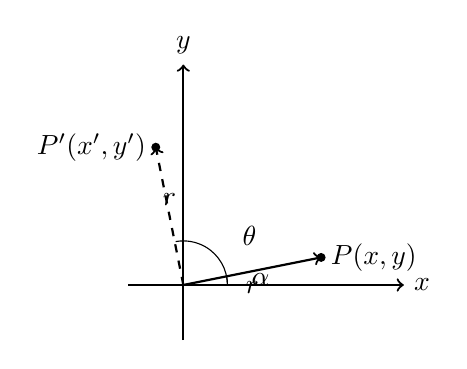
\begin{tikzpicture}[scale=0.7]
\draw[->,thick] (-1,0) -- (4,0) node[right]{$x$};
\draw[->,thick] (0,-1) -- (0,4) node[above]{$y$};
\filldraw (2.5,0.5) circle (2pt) node[right]{$P(x,y)$};
\filldraw (-0.5,2.5) circle (2pt) node[left]{$P'(x',y')$};
\draw[->,thick] (0,0) -- (2.5,0.5) node[midway,below]{$r$};
\draw[->,thick,dashed] (0,0) -- (-0.5,2.5) node[midway,above]{$r$};
\draw (0.8,0) arc (0:12:0.8);
\node at (1.4,0.1){$\alpha$};
\draw (0.8,0) arc (0:100:0.8);
\node at (1.2,0.9){$\theta$};
\end{tikzpicture}
\end{center}

\begin{exercise}
\item 用公式计算，不凭直觉：点$(3,0)$转$90^\circ$后到哪？转$270^\circ$后呢？
\item 用公式计算：点$(2,1)$转$180^\circ$后坐标是？
\item 用公式计算：点$(4,3)$转$90^\circ$后坐标是？
\item $\theta=45^\circ$时，计算$(1,0)$的像。($\cos45^\circ=\sin45^\circ=\frac{\sqrt2}{2}$)
\item 点$(1,1)$先转$90^\circ$，再对结果转$90^\circ$，再转$90^\circ$，再转$90^\circ$，写出每一步的坐标。旋转$360^\circ$后是否回到原位？用公式说明。
\item 写出点$(x,y)$绕原点顺时针旋转$90^\circ$（即$\theta=-90^\circ$）后的坐标。提示：$\cos(-90^\circ)=0$，$\sin(-90^\circ)=-1$。
\end{exercise}

\sectiontitle{1.3\quad 反射变换}

\textbf{定义}：设$l$是平面上一条直线。对于平面上任意一点$P$，过$P$作$l$的垂线，垂足为$H$。在射线$PH$的反向延长线上取一点$P'$，使得$HP' = PH$。则称点$P'$为点$P$关于直线$l$的反射像，这个对应关系称为关于$l$的反射变换（或轴对称变换），直线$l$称为对称轴。

简而言之：反射变换把一个点翻折到直线的另一侧，翻折前后该点到直线的距离不变，且连线垂直于对称轴。

\begin{center}
\begin{tikzpicture}[scale=0.7]
  \draw[->,thick] (-1,0) -- (5,0) node[right]{$x$};
  \draw[->,thick] (0,-3) -- (0,3) node[above]{$y$};
  \draw[densely dashed, gray] (3,2) -- (3,-2);
  \filldraw (3,2) circle (2.5pt) node[above right]{$P(3,2)$};
  \filldraw (3,-2) circle (2.5pt) node[below right]{$P'(3,-2)$};
  \filldraw (3,0) circle (1.5pt) node[below right]{$H$};
  \node at (3.3,1){$2$};
  \node at (3.3,-1){$2$};
\end{tikzpicture}
\end{center}

现在我们通过具体计算来看这个定义在坐标平面上怎么操作。先看关于$x$轴的反射。

\textbf{关于$x$轴的反射}：对称轴$l$是$x$轴（即直线$y=0$）。取点$P(3,2)$，它到$x$轴的距离是$|2|=2$。过$P$作$x$轴的垂线（竖直线$x=3$），垂足$H=(3,0)$。在$H$的另一侧取$P'$使$HP'=2$，即$P'=(3,-2)$。所以$(3,2)$关于$x$轴反射的像是$(3,-2)$。

再算几个：
\begin{itemize}
\item $(-1,4)$：到$x$轴距离$4$，垂线$x=-1$，垂足$(-1,0)$，反射像$(-1,-4)$。
\item $(5,0)$：到$x$轴距离$0$，点就在轴上，反射像就是它自己$(5,0)$。
\item $(2,-3)$：距离$3$，反射到轴上方$(2,3)$。
\end{itemize}

\begin{example}
从以上例子，归纳关于$x$轴反射的坐标规律。
\end{example}
\begin{solution}
每个点的$x$坐标完全不变，$y$坐标变成了它的相反数。规律是：
\[
x'=x,\quad y'=-y
\]
\end{solution}

\textbf{关于$y$轴的反射}：对称轴是$y$轴。用同样的方法分析：
\begin{itemize}
\item $(3,2)$：到$y$轴距离$3$，反射到$y$轴左侧$(-3,2)$。
\item $(5,-1)$：到$y$轴距离$5$，反射像$(-5,-1)$。
\item $(0,4)$：在$y$轴上，反射像$(0,4)$就是它自己。
\end{itemize}

\begin{example}
归纳关于$y$轴反射的坐标规律。
\end{example}
\begin{solution}
$y$坐标不变，$x$坐标取相反数：$x'=-x$，$y'=y$。
\end{solution}

\textbf{关于直线$y=x$的反射}：点$(3,2)$关于$y=x$的反射像是什么样子的？根据定义，$(3,2)$到直线$y=x$的垂线方程为$y-2=-(x-3)$，整理得$y=5-x$。这条垂线和$y=x$的交点（即垂足）是$(\frac52,\frac52)$。从$(3,2)$到垂足$(\frac52,\frac52)$的向量是$(-\frac12,\frac12)$，从垂足反方向走同样的距离，得到反射像$(2,3)$。

发现了吗？$(3,2)$关于$y=x$的反射像是$(2,3)$——就是把两个坐标对调了。再验证一个：$(4,1)$关于$y=x$的反射像应该是对调坐标得到$(1,4)$。我们来算：垂线$y-1=-(x-4)$交$y=x$于$(\frac52,\frac52)$，反射后确实是$(1,4)$。

继续验证：
\begin{itemize}
\item $(-1,3)$关于$y=x$反射：$(3,-1)$。
\item $(5,-2)$关于$y=x$反射：$(-2,5)$。
\end{itemize}

\begin{example}
归纳关于$y=x$反射的坐标规律。
\end{example}
\begin{solution}
$x$和$y$坐标互换：$x'=y$，$y'=x$。
\end{solution}

\textbf{关于直线$y=-x$的反射}：用同样的方法可以导出规律。$(3,2)$关于$y=-x$的反射像是$(-2,-3)$——坐标互换且都取相反数：
\[
x'=-y,\quad y'=-x
\]

最后注意一个性质：反复做两次同一个反射会回到原位。这是因为第一次反射把点翻到另一侧，第二次又翻回来了。你可以拿任何坐标验证：比如$(3,2)$关于$x$轴反射→$(3,-2)$→再反射一次→$(3,2)$。

\begin{exercise}
\item 点$(5,-3)$关于$x$轴对称后到哪？用$y$坐标取反的规则计算，然后画图验证。
\item 点$(-2,4)$关于$y$轴对称后到哪？
\item 分别计算$(4,1)$关于$y=x$和关于$y=-x$的反射像。
\item 点$A(2,3)$先关于$x$轴反射，再关于$y$轴反射，最终坐标是多少？这个结果相当于做了一个什么变换？提示：和$(2,3)$关于原点对称（即旋转$180^\circ$）的结果比较。
\item 点$B(1,0)$按照"关于$y=x$反射→关于$x$轴反射"的顺序做复合变换，写出每一步的坐标。
\end{exercise}

\sectiontitle{1.4\quad 伸缩变换}

\textbf{定义}：沿$x$轴方向拉伸$k$倍（$k\neq0$）的伸缩变换，是指把每个点的$x$坐标乘以$k$，$y$坐标保持不变。若$|k|>1$则拉长，$|k|<1$则缩短，$k<0$则拉伸到另一侧。

\begin{center}
\begin{tikzpicture}[scale=0.7]
  \draw[->,thick] (-1,0) -- (7,0) node[right]{$x$};
  \draw[->,thick] (0,-1) -- (0,5) node[above]{$y$};
  % Original square
  \draw[gray, thick, fill=lightblue!30] (0,0) rectangle (2,3);
  \node[gray] at (1,1.5){原正方形};
  % Stretched rectangle
  \draw[mainblue, thick] (0,0) rectangle (6,3);
  \node[mainblue] at (3,1.5){$k=3$拉伸后};
  \node at (3,-0.5){$x$方向拉伸$3$倍：$1\times1\to3\times1$};
\end{tikzpicture}
\end{center}

\begin{itemize}
\item $k=2$时：$(1,2)\to(2,2)$，$(3,1)\to(6,1)$，$(-1,3)\to(-2,3)$。注意$x$坐标都变成了原来的两倍。
\item $k=\frac12$时：$(4,3)\to(2,3)$，$(6,5)\to(3,5)$。$x$方向被压扁了一半。
\item $k=-2$时：$(1,2)\to(-2,2)$。$x$坐标不仅拉长了两倍，还翻到了$y$轴的另一边。
\end{itemize}

从这些例子归纳公式：$x'=kx$，$y'=y$。

同理，沿$y$轴方向拉伸$l$倍（$l\neq0$）：$x'=x$，$y'=ly$。

两个方向可以同时拉伸：$x'=kx$，$y'=ly$。

\begin{example}
举例：$k=2,l=3$时，$(1,1)$变成多少？原来的$1\times1$正方形变成了什么样的形状？面积变成了原来的几倍？
\end{example}
\begin{solution}
$(1,1)\to(2,3)$。正方形的四个顶点$(0,0),(1,0),(1,1),(0,1)$分别变成$(0,0),(2,0),(2,3),(0,3)$，是一个$2\times3$的矩形。面积$=2\times3=6$，是原来的$6$倍。
\end{solution}

\begin{exercise}
\item 计算：点$(4,5)$沿$x$方向拉伸$3$倍后到哪？沿$y$方向压缩到$\frac12$倍呢？
\item 点$(-2,5)$沿$x$方向拉伸$-1$倍，结果是什么？这和哪种变换效果相同？
\item $k=3,l=4$时，计算$(2,1)$的像。这个变换把面积放大了几倍？
\item 先沿$x$拉伸$2$倍，再沿$y$拉伸$3$倍。和先做$y$再做$x$的结果一样吗？取一个点算一下。
\item 沿$x$方向拉伸$2$倍后，能不能再做一个伸缩变换把图形恢复到原样？如果能，怎么做？
\end{exercise}

\sectiontitle{1.5\quad 投影变换}

\textbf{定义}：向$x$轴的投影变换，是指把每个点$(x,y)$映射为$(x,0)$。即保留横坐标，丢弃纵坐标。

\begin{itemize}
\item $(3,5)\to(3,0)$，$(3,-2)\to(3,0)$，$(-1,4)\to(-1,0)$。
\end{itemize}

注意，$(3,5)$和$(3,-2)$是两个完全不同的点，但它们的投影相同——都是$(3,0)$。这意味着从投影结果无法唯一确定原始的点。因此投影变换是不可逆的。

向$y$轴的投影：$x'=0$，$y'=y$。$(3,5)\to(0,5)$，$(-2,5)\to(0,5)$——$(-2,5)$和$(3,5)$投影后重合。

公式：
\begin{align*}
\text{向$x$轴投影}&: x'=x,\; y'=0\\
\text{向$y$轴投影}&: x'=0,\; y'=y
\end{align*}

\begin{example}
把单位正方形（顶点$(0,0),(1,0),(1,1),(0,1)$）分别向$x$轴和$y$轴投影。投影后的图形各是什么？
\end{example}
\begin{solution}
向$x$轴投影：四个顶点都变成$(0,0),(1,0),(1,0),(0,0)$——实际上退化为$x$轴上从$(0,0)$到$(1,0)$的线段。\\
向$y$轴投影：四个顶点变成$(0,0),(0,0),(0,1),(0,1)$——退化为$y$轴上从$(0,0)$到$(0,1)$的线段。
\end{solution}

\begin{exercise}
\item 点$(4,-3)$向$x$轴投影后到哪？向$y$轴投影后到哪？
\item 点$(2,5)$和$( -2,5)$向$y$轴投影后是否重合？$(2,5)$和$(2,-5)$向$x$轴投影后是否重合？
\item 为什么投影变换不可逆？从几何上说明。
\end{exercise}

\sectiontitle{1.6\quad 切变变换}

\textbf{定义}：沿$x$方向的切变变换（系数为$k$）是指把每个点$(x,y)$映射为$(x+ky,y)$。其中$y$坐标不变，$x$坐标上额外增加一个与$y$成正比的量。

试几个具体数字：
\begin{itemize}
\item $k=2$，点$(1,2)$：$x'=1+2\times2=5$，$y'=2$，变成$(5,2)$。
\item $k=2$，点$(3,0)$：$x'=3+2\times0=3$，$y'=0$，没变。因为$y=0$，不受切变影响。
\item $k=2$，点$(2,3)$：$x'=2+2\times3=8$，$y'=3$，变成$(8,3)$。
\item $k=-2$，点$(1,3)$：$x'=1+(-2)\times3=-5$，$y'=3$，变成$(-5,3)$。$k$为负时往左推。
\end{itemize}

把单位正方形做$k=1$的切变，看看形状怎么变。四个顶点：
\begin{align*}
A(0,0) &\to (0+1\times0,0)=(0,0)\\
B(1,0) &\to (1+1\times0,0)=(1,0)\\
C(1,1) &\to (1+1\times1,1)=(2,1)\\
D(0,1) &\to (0+1\times1,1)=(1,1)
\end{align*}
新顶点为$(0,0),(1,0),(2,1),(1,1)$——原来的正方形变成了一个平行四边形。注意底边长仍是$1$，高仍是$1$，所以面积没有变化。这是一个重要的性质，会在第三章中专门讨论。

\begin{center}
\begin{tikzpicture}[scale=1.2]
  \draw[->,thick] (-0.5,0) -- (3,0) node[right]{$x$};
  \draw[->,thick] (0,-0.5) -- (0,2) node[above]{$y$};
  % Original square
  \draw[gray, thick, dashed, fill=lightblue!20] (0,0) rectangle (1,1);
  \node[gray] at (0.5,0.5){正方形};
  % Sheared parallelogram
  \draw[mainblue, thick, fill=mainblue!10] (0,0) -- (1,0) -- (2,1) -- (1,1) -- cycle;
  \node[mainblue] at (1.2,0.4){平行四边形};
  \node at (1.2,-0.4){底$=1$，高$=1$，面积不变};
\end{tikzpicture}
\end{center}

\begin{exercise}
\item $k=3$时，计算$(1,2)$和$(1,0)$切变后的坐标。为什么$(1,0)$不变？
\item $k=-2$时，计算$(1,3)$切变后的坐标。负$k$意味着往哪个方向推？
\item 单位正方形的四个顶点做$k=3$的切变后，新顶点坐标各是什么？
\item 做一次$k=2$的切变后，再做一个什么参数的切变能把图形变回去？算一下验证。
\item 沿$y$方向的切变公式应该是怎样的？猜测并验证一个例子。
\end{exercise}

\sectiontitle{1.7\quad 本章小结}

我们已经见过五种变换：旋转、反射、伸缩、投影、切变。注意，每种变换的公式都写成
\[
x' = ax + by,\qquad y' = cx + dy
\]
的形式（平移是个例外，将在第五章处理）。它们的区别仅在于$a,b,c,d$分别取了什么数。

\begin{exercise}
\item 点$(3,4)$绕原点逆时针旋转$90^\circ$，再关于$x$轴反射。用每一步的公式计算最终坐标。
\item 点$(-1,5)$先关于$y=x$反射，再沿$x$方向拉伸$2$倍。写出每一步的坐标。
\item 点$(5,0)$做$x$方向$k=2$的切变，然后向$y$轴投影。最终坐标是什么？
\item 正方形顶点$(0,0),(2,0),(2,2),(0,2)$依次经过以下变换，逐步计算每个变换后的新顶点：\\
(a) 关于$x$轴反射\\
(b) 沿$y$方向拉伸$2$倍\\
(c) $x$方向$k=1$的切变\\
(d) 旋转$180^\circ$
\item 判断，并说明理由：\\
(a) 旋转变换保持两点间的距离不变吗？\\
(b) 投影变换可逆吗？\\
(c) 切变变换改变面积吗？\\
(d) 任何反射变换做两次等于恒等变换（什么都不变）吗？
\item 哪种变换能把正方形变成长方形？哪种能把正方形变成面积不变的平行四边形？
\item 思考：为什么线性变换的公式只能是$ax+by$而不能含$x^2$或$\sqrt{x}$？提示：直线经过这样的变换后，还应该是直线吗？
\end{exercise}

\sectiontitle{课后练习}

\subsection*{A组\quad 基础巩固}

\begin{exercise}
\item 点$(7,-2)$绕原点逆时针旋转$90^\circ$，求旋转后的坐标。
\item 点$(-4,6)$关于$x$轴对称后到哪？关于$y=x$对称后呢？
\item 点$(1.5,\,0)$做$x$方向拉伸$4$倍，再关于$y$轴对称，求最终坐标。
\item 点$(3,-1)$做$x$方向$k=-2$的切变，求变换后的坐标。向$x$轴投影后呢？
\item 单位正方形的四个顶点$(0,0),(1,0),(1,1),(0,1)$做旋转$270^\circ$，求四个新顶点坐标。
\item 点$A(2,5)$先旋转$180^\circ$，再关于$x$轴反射，再沿$x$方向拉伸$3$倍。求最终坐标。
\item 写出下列变换的公式：(a) 旋转$90^\circ$；(b) 关于$y=-x$反射；(c) $x$拉伸$\frac12$倍、$y$拉伸$3$倍。
\item 点$P$经旋转$90^\circ$后得到$(2,-3)$，求$P$的原坐标。
\item 判断下列变换是否可逆，并说明理由：旋转变换、向$x$轴投影、切变变换。
\item 一个点经三次关于$x$轴的反射，结果相当于做了什么变换？
\end{exercise}

\subsection*{B组\quad 挑战提升}

\begin{exercise}
\item 点$(1,\sqrt3)$绕原点逆时针旋转$30^\circ$，求旋转后的坐标。（提示：$\cos30^\circ=\frac{\sqrt3}{2}$，$\sin30^\circ=\frac12$。）
\item 写出关于直线$x=2$对称的变换公式。（提示：先平移坐标系把$x=2$变到$y$轴，反射，再平移回去——或者直接从定义推导。）
\item 旋转$\theta$后再旋转$-\theta$，结果回到了原位。用旋转公式代数验证这一点。
\item 两个旋转变换的复合：先旋转$\theta_1$再旋转$\theta_2$，总效果是什么？写出复合变换的坐标公式。
\item 能否找到两个不同的反射变换，它们的复合结果是一个旋转变换？如果能，写出具体的例子。
\item 某变换满足：$(1,0)\to(0,2)$，$(0,1)\to(-3,0)$，$(1,1)\to(-3,2)$。这个变换是哪种类型？写出它的公式。
\item 点$(3,5)$依次经过以下变换，求最终坐标：先绕原点逆时针旋转$135^\circ$，再关于$y=x$反射，最后沿$x$方向拉伸$\frac13$倍。\\
（提示：$\cos135^\circ=-\frac{\sqrt2}{2}$，$\sin135^\circ=\frac{\sqrt2}{2}$。）
\item 一个正方形顶点为$(0,0),(2,0),(2,2),(0,2)$，先做$x$方向$k=1.5$的切变，再绕原点旋转$45^\circ$。写出旋转后的四个顶点坐标（保留根号）。
\item 某点经过某种变换后到达$(5,-2)$。已知该变换是先沿$y$方向拉伸$3$倍，再关于直线$y=-x$反射。求原点的坐标。
\item 能否找到一个变换，它既不是单纯的旋转、反射、伸缩、投影、切变中的任何一种，但却是这五种中某两种的复合？举一个具体的坐标公式例子，并用一个点验证。
\end{exercise}

\newpage
